

\tikzset{every picture/.style={line width=0.75pt}} %set default line width to 0.75pt        

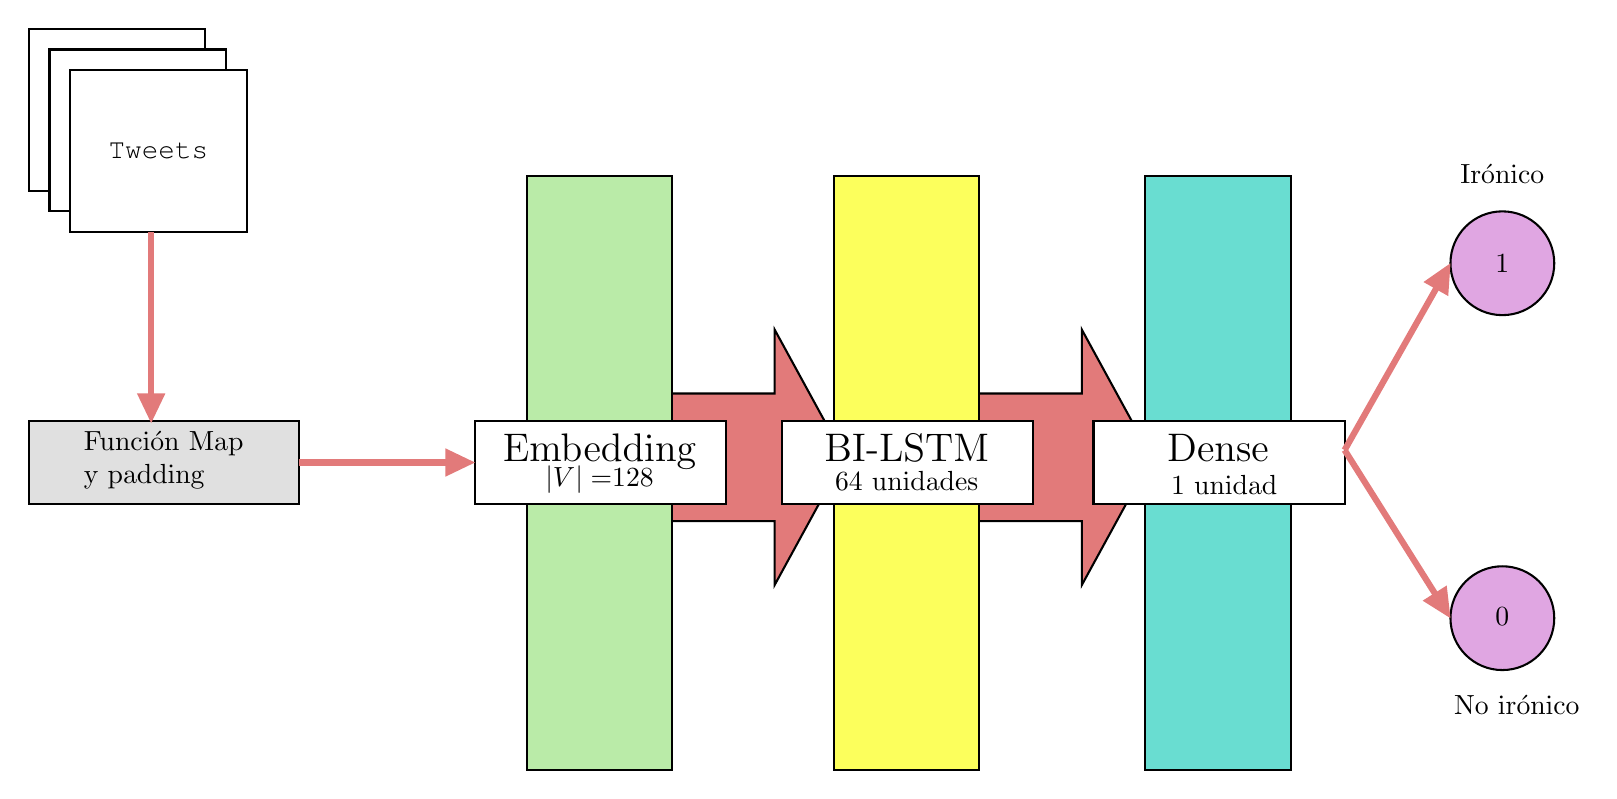
\begin{tikzpicture}[x=0.75pt,y=0.75pt,yscale=-1,xscale=1]
%uncomment if require: \path (0,560); %set diagram left start at 0, and has height of 560

%Right Arrow [id:dp8310111909351754] 
\draw  [fill={rgb, 255:red, 226; green, 122; blue, 122 }  ,fill opacity=1 ] (557,229.75) -- (607.4,229.75) -- (607.4,199) -- (641,260.5) -- (607.4,322) -- (607.4,291.25) -- (557,291.25) -- cycle ;
%Right Arrow [id:dp47914845862025834] 
\draw  [fill={rgb, 255:red, 226; green, 122; blue, 122 }  ,fill opacity=1 ] (409,229.75) -- (459.4,229.75) -- (459.4,199) -- (493,260.5) -- (459.4,322) -- (459.4,291.25) -- (409,291.25) -- cycle ;
%Shape: Rectangle [id:dp6690480869865736] 
\draw  [fill={rgb, 255:red, 186; green, 235; blue, 168 }  ,fill opacity=1 ] (340,125) -- (410,125) -- (410,411) -- (340,411) -- cycle ;
%Shape: Rectangle [id:dp5000001257312081] 
\draw  [fill={rgb, 255:red, 255; green, 255; blue, 255 }  ,fill opacity=1 ] (315,243) -- (436,243) -- (436,283) -- (315,283) -- cycle ;

%Shape: Rectangle [id:dp10129983649453078] 
\draw  [fill={rgb, 255:red, 252; green, 255; blue, 92 }  ,fill opacity=1 ] (488,125) -- (558,125) -- (558,411) -- (488,411) -- cycle ;
%Shape: Rectangle [id:dp5417230650141682] 
\draw  [fill={rgb, 255:red, 255; green, 255; blue, 255 }  ,fill opacity=1 ] (463,243) -- (584,243) -- (584,283) -- (463,283) -- cycle ;

%Shape: Rectangle [id:dp3694545240809384] 
\draw  [fill={rgb, 255:red, 105; green, 221; blue, 209 }  ,fill opacity=1 ] (638,125) -- (708,125) -- (708,411) -- (638,411) -- cycle ;
%Shape: Rectangle [id:dp46595094502729073] 
\draw  [fill={rgb, 255:red, 255; green, 255; blue, 255 }  ,fill opacity=1 ] (613,243) -- (734,243) -- (734,283) -- (613,283) -- cycle ;

%Shape: Rectangle [id:dp8981854115946217] 
\draw  [fill={rgb, 255:red, 255; green, 255; blue, 255 }  ,fill opacity=1 ] (100,54) -- (185,54) -- (185,132) -- (100,132) -- cycle ;
%Shape: Rectangle [id:dp3678809591192025] 
\draw  [fill={rgb, 255:red, 255; green, 255; blue, 255 }  ,fill opacity=1 ] (110,64) -- (195,64) -- (195,142) -- (110,142) -- cycle ;
%Shape: Rectangle [id:dp18627809361061853] 
\draw  [fill={rgb, 255:red, 255; green, 255; blue, 255 }  ,fill opacity=1 ] (120,74) -- (205,74) -- (205,152) -- (120,152) -- cycle ;

%Shape: Rectangle [id:dp5391508691442917] 
\draw  [fill={rgb, 255:red, 224; green, 224; blue, 224 }  ,fill opacity=1 ] (100,243) -- (230,243) -- (230,283) -- (100,283) -- cycle ;

%Straight Lines [id:da3222212402232878] 
\draw [color={rgb, 255:red, 226; green, 122; blue, 122 }  ,draw opacity=1 ][line width=2.25]    (230,263) -- (311,263) ;
\draw [shift={(315,263)}, rotate = 180] [fill={rgb, 255:red, 226; green, 122; blue, 122 }  ,fill opacity=1 ][line width=2.25]  [draw opacity=0] (14.29,-6.86) -- (0,0) -- (14.29,6.86) -- cycle    ;

%Shape: Circle [id:dp5889762673635599] 
\draw  [fill={rgb, 255:red, 224; green, 166; blue, 226 }  ,fill opacity=1 ] (785,167) .. controls (785,153.19) and (796.19,142) .. (810,142) .. controls (823.81,142) and (835,153.19) .. (835,167) .. controls (835,180.81) and (823.81,192) .. (810,192) .. controls (796.19,192) and (785,180.81) .. (785,167) -- cycle ;
%Shape: Circle [id:dp18063293168467354] 
\draw  [fill={rgb, 255:red, 224; green, 166; blue, 226 }  ,fill opacity=1 ] (785,338) .. controls (785,324.19) and (796.19,313) .. (810,313) .. controls (823.81,313) and (835,324.19) .. (835,338) .. controls (835,351.81) and (823.81,363) .. (810,363) .. controls (796.19,363) and (785,351.81) .. (785,338) -- cycle ;
%Straight Lines [id:da9689497769272035] 
\draw [color={rgb, 255:red, 226; green, 122; blue, 122 }  ,draw opacity=1 ][line width=2.25]    (734,257) -- (783.03,170.48) ;
\draw [shift={(785,167)}, rotate = 479.54] [fill={rgb, 255:red, 226; green, 122; blue, 122 }  ,fill opacity=1 ][line width=2.25]  [draw opacity=0] (14.29,-6.86) -- (0,0) -- (14.29,6.86) -- cycle    ;

%Straight Lines [id:da9360660330658093] 
\draw [color={rgb, 255:red, 226; green, 122; blue, 122 }  ,draw opacity=1 ][line width=2.25]    (734,257) -- (782.87,334.62) ;
\draw [shift={(785,338)}, rotate = 237.8] [fill={rgb, 255:red, 226; green, 122; blue, 122 }  ,fill opacity=1 ][line width=2.25]  [draw opacity=0] (14.29,-6.86) -- (0,0) -- (14.29,6.86) -- cycle    ;

%Straight Lines [id:da7770649855526097] 
\draw [color={rgb, 255:red, 226; green, 122; blue, 122 }  ,draw opacity=1 ][line width=2.25]    (159,152) -- (159,240) ;
\draw [shift={(159,244)}, rotate = 270] [fill={rgb, 255:red, 226; green, 122; blue, 122 }  ,fill opacity=1 ][line width=2.25]  [draw opacity=0] (14.29,-6.86) -- (0,0) -- (14.29,6.86) -- cycle    ;


% Text Node
\draw (375,264) node  [align=left] {{\Large Embedding}\\};
% Text Node
\draw (523,264) node  [align=left] {{\Large BI-LSTM}\\};
% Text Node
\draw (673,264) node  [align=left] {{\Large Dense}\\};
% Text Node
\draw (375,271) node  [align=left] {$\displaystyle |V|=$128};
% Text Node
\draw (523,272) node  [align=left] {64 unidades};
% Text Node
\draw (676,274) node  [align=left] {1 unidad};
% Text Node
\draw (162.5,113) node  [align=left] {{\fontfamily{pcr}\selectfont Tweets}};
% Text Node
\draw (165,262) node  [align=left] {Función Map\\y padding};
% Text Node
\draw (810,167) node  [align=left] {1};
% Text Node
\draw (810,337) node  [align=left] {0};
% Text Node
\draw (810,124) node  [align=left] {Irónico};
% Text Node
\draw (817,380) node  [align=left] {No irónico};


\end{tikzpicture}
